\documentclass[a4paper]{article}
\usepackage[francais]{babel}
\usepackage[utf8]{inputenc}

\usepackage{graphicx}
\usepackage{fancyhdr}
\usepackage{lastpage}
\usepackage{amsmath}
\usepackage{xspace}
\usepackage{textcomp}

\usepackage{hyperref}

\usepackage[top=30mm, bottom=30mm, left=25mm, right=25mm]{geometry}

\pagestyle{fancy}

\usepackage{helvet}

\usepackage{verbatim}
\usepackage{amsmath}
\usepackage[table]{xcolor}
\definecolor{bleugris}{rgb}{.2,.4,.5}

\definecolor{colKeys}{rgb}{0,0,1} 
\definecolor{colIdentifier}{rgb}{0,0,0} 
\definecolor{colComments}{rgb}{0,0.5,1} 
\definecolor{colString}{rgb}{0.6,0.1,0.1} 

\usepackage{listings}

% Permet l'ajout de code par insertion du fichier le contenant
% Les arguments sont :
% $1 : nom du fichier à inclure
% $2 : le type de langage (C++, C, Java ...)
\newcommand{\addCode}[2]{%

  % Configuration de la coloration syntaxique du code
  \definecolor{colKeys}{rgb}{0,0,1}
  \definecolor{colIdentifier}{rgb}{0,0,0}
  \definecolor{colComments}{rgb}{0,0.5,1}
  \definecolor{colString}{rgb}{0.6,0.1,0.1}

  % Configuration des options 
  \lstset{%
    language = #2,%
    identifierstyle=\color{colIdentifier},%
    basicstyle=\ttfamily\scriptsize, %
    keywordstyle=\color{colKeys},%
    stringstyle=\color{colString},%
    commentstyle=\color{colComments},%
    columns = flexible,%
    %tabsize = 8,%
    showspaces = false,%
    numbers = left, numberstyle=\tiny,%
    frame = single,frameround=tttt,%
    breaklines = true, breakautoindent = true,%
    captionpos = b,%
    xrightmargin=10mm, xleftmargin = 15mm, framexleftmargin = 7mm,%
  }%
    \begin{center}
    \lstinputlisting{#1}
    \end{center}
}

\newcommand{\nTitle}[1]{%
	\clearpage
	\vspace*{\fill}		%
	\begin{center}	%
		\part{#1}		%
	\end{center}
	\vspace*{\fill}		%
	\clearpage
}

\newenvironment{nAbstract} 		%
{ 								%
	\newpage 					% 
	\vspace*{\fill}				%
	\begin{center}			 	%
		\begin{abstract}		%
}{								%
		\end{abstract}			%
	\end{center}				%
	\vspace*{\fill}				%
	\newpage					%
}


\newcommand{\nClass}[1]{{\color{bleugris}{\textsl{\textbf{#1}}}}}
\newcommand{\nParameter}[1]{{\color{gray}{\textbf{#1}}}}
\newcommand{\nMethod}[1]{{\color{gray}{\textbf{#1}}}}
\newcommand{\nConstant}[1]{\texttt{\uppercase{#1}}}
\newcommand{\nKeyword}[1]{\textsl{\textbf{#1}}}

\graphicspath{{../SourcesMatlab/}}

% Conversion nombres arabes / romain
\makeatletter
\newcommand{\rmnum}[1]{\romannumeral #1}
\newcommand{\Rmnum}[1]{\expandafter\@slowromancap\romannumeral #1@}
\makeatother

\setlength{\headheight}{14pt}

\fancyhf{}


\makeatletter
\def\clap#1{\hbox to 0pt{\hss #1\hss}}%
\def\ligne#1{%
\hbox to \hsize{%
\vbox{\centering #1}}}%
\def\haut#1#2#3{%
\hbox to \hsize{%
\rlap{\vtop{\raggedright #1}}%
\hss
\clap{\vtop{\centering #2}}%
\hss
\llap{\vtop{\raggedleft #3}}}}%
\def\bas#1#2#3{%
\hbox to \hsize{%
\rlap{\vbox{\raggedright #1}}%
\hss
\clap{\vbox{\centering #2}}%
\hss
\llap{\vbox{\raggedleft #3}}}}%
\def\maketitle{%
\thispagestyle{empty}\vbox to \vsize{%
\vfill
\vspace{1cm}
\begin{flushleft}
\usefont{OT1}{ptm}{m}{n}
\huge \@title
\end{flushleft}
\par
\hrule height 4pt
\par
\begin{flushright}
\usefont{OT1}{phv}{m}{n}
\Large \@author
\par
\end{flushright}
\vspace{1cm}
\vfill
\vfill
\bas{}{\@blurb \vspace{1cm}}{}
}%
\cleardoublepage
}
\def\date#1{\def\@date{#1}}
\def\author#1{\def\@author{#1}}
\def\title#1{\def\@title{#1}}
\def\blurb#1{\def\@blurb{#1}}
\author{}
\title{}
\blurb{}
\makeatother


\usepackage{hyperref}
\hypersetup{
colorlinks=false, % bool: Liens colorés
pdfborder={0 0 0} % Ne pas encadrer les liens
}

\usepackage[final]{pdfpages}
\usepackage{rotating}
\usepackage{eurosym}
\usepackage{lscape}
\usepackage{float}
\usepackage{color}
\usepackage{colortbl}
\usepackage{array}
\usepackage[printonlyused]{acronym}

% définir les commandes ici

% s'il y a beaucoup de commandes et de packages à inclure n'h&ésitez pas
% à mettre tout ça dans un fichier include.tex et l'inclure
% \input{include.tex}

\lhead{PdC4 - Choix d'une architecture informatique}
\rhead{
\includegraphics [width=1.5cm]{insa-couleur.jpg}}
\rfoot{\thepage\ de \pageref{LastPage}}



\begin{document}
\title{PdC 4 : Veille technologique : Outils d'aide au pilotage}
\author{Elisa ABIDH, Adrien BROCHOT, Julien LEVESY,Armand ROSSIUS}

%------------------------------------- Page de titre
\maketitle
%\begin{titlepage}
%~

%\vfill
%\begin{Large}
%Septembre 2011
%\end{Large}
%\vfill
%\end{titlepage}
%----------------------------------------------------

%--------------------------------- Table des matières
\newpage
\tableofcontents
\newpage
%----------------------------------------------- Plan

\section{Enjeu de l'informatique décisionnelle}
Nous vivons dans un monde ou chaque action, chaque opération génère des données Cette assertion s'applique évidement au monde de l'entreprise, ou l’activité est plus que jamais organisée et formalisée sous formes de processus.
A chaque étape du processus métier, un quotta de donnée est généré de façon à tracer l’activité de l’entreprise. Ces données peuvent être de plusieurs types, références, fournisseurs ou encore analytiques.\\
Malheureusement, ce rapport à la donnée amène la constitution de gigantesque “DataWarehouses”, ou entrepôts de données possédant une telle complexité et multiplicité qu’ils en deviennent inexploitables. Sans interprétation, traitement et exploitation préalable il devient impossible de déduire quelque chose de ces entrepôts de données.\\
Le besoin est donc clair, il faut “donner” de la visibilité à ces entrepôts de données. Ainsi, par la définitions de différents tableau d’indicateurs synthétiques et pertinents, il deviens facile d’exploiter les données collectées. Ceci est particulièrement destiné au public de décideurs, non informaticiens... \\
Plus loin encore, certains procédés permettent de générée des données à partir d’autres données de masses. En effet en isolant des tendances, des modèles d’actions entre les différentes entités, nous sommes en mesure d'obtenir de nouvelles informations insoupçonnées.\\
C’est ici qu'interviennent les solutions de business intelligence, ou informatique décisionnelle. Par ce terme, il est désigné l'ensemble des outils ou méthodes appliquées à la donnée, depuis sa collecte, jusqu’à la définition de “tableau de bords” à destination des décideurs.
Ainsi nous pouvons isoler les étapes suivantes :
\begin{itemize}
\item[•]Collecte : Cette phase englobe les étapes d'extraction des données, de traitement et enfin chargée dans l'entrepôt de données. Elles est plus souvent déléguée à des outils type ETL fournis par des grands acteurs du domaine.
\item[•]Intégration : Il ne suffit pas de charger les données pour les rendre exploitables. Ainsi tout un procédé de nettoyage, synchronisation avec les données actuelles, et enfin de certification. Sans cette étape, la pérennité de l'entrepôt de données serait mise en question par un grand nombre de données incorrectes / corrompues et surtout non exploitables.
\item[•]Distribution : Du fait de la taille de l'entrepôt de données, il est impossible de traiter la globalité des données, ainsi, le regroupement des données et la distribution en sous ensemble cohérents d’un point de vue opérationnel, (ie un regroupement par secteur...)  est nécessaire, de façon à optimiser les temps de traitements des diverses applications exploitant ces données.
\item[•]Présentation : Sous la forme d’indicateurs concrets, voire de tableaux de bord classiques, les données sont exprimées de manière à ce que n’importe quel utilisateur final puisse les comprendre et en tenir compte dans les décisions de la façon la plus complète possible.
\item[•]Administration :  Des fonctionnalités d’administration du DataWarehouse, de son alimentation, une gestion des compte / application utilisatrices de ces données, impliquant un contrôle d’accès, de répartition de la charge et autres implications importantes délégués au contrôle des systèmes de données de grande envergure.
\end{itemize}

\begin{figure}[H]
\begin{center}
  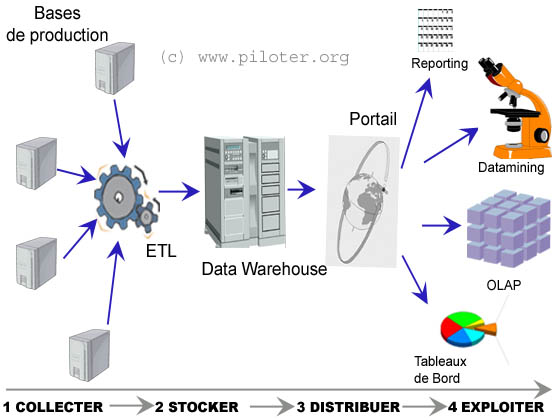
\includegraphics[scale= 0.5]{Enjeu.jpg}
  \caption{Les 4 phases du processus de Business Intelligence : de la donnée à l'information.}
\end{center}  
\end{figure}

\section{Solutions orientées SOA}
La logique même du SOA est de fournir à un SI la capacité à se développer en adjoignant une logique de composants au SI. Ainsi, il est cohérent d’envisager la piste du déploiement d’une solution de business intelligence dans une démarche SOA.\\
Les composants clés de ces systèmes sont :
\begin{itemize}
\item[•]EAI : Enterprise Application Integration  : Système de communication entre les différentes applications opérationelles, visant à assurer la cohérence entre le DW et les différentes bases de données opérationelles, déployées chez l’utilisateur.
\item[•]Master Data Management :  (Optionnel, mais potentiellement critique à long terme )  Système d’optimisaiton de la qualité basé sur la création d’un sous enssemble de données de références au plus justes possibles, permettant à long terme de garantir la qualité des données et une cohérence dans l’exploitation des données transactionnelles
\item[•]ETL : Extract, Transform, Load : Directement Raccordé à l’EAI, il s’agit d’un utilitiare la encore basées sur les Métadonnées, qui permet d’assurer l’extraction, l’uniformisation et la structuration des données issurées des BDD opérationelles, et leur chargement  / intégration au sein du Data Warehouse et des datamarts.
\item[•] DataWarehouse  : Schéma de BDD central, servant de base d’exploitation aux outils de  BI.
\item[•] Solutions de BI intégrées : Présentation, Reporting et exploitation : 
\end{itemize}
Principaux acteurs du marché :
\begin{itemize}
\item[•]Oracle
\item[•]IBM
\end{itemize}  
\section{Solution internet : BITTLE}
Bittle est une solution décisionnelle, accesible par le web selon le modèle SaaS (Software as a Service). Bittle permet de construire des tableaux de bord et reporting en ligne grâce au suivi d'indicateurs. On peut donc retrouver l'ensemble des fonctionnalités de cette solution à l'adresse internet suivante :  www.bittle-solutions.com . L'offre qu'elle propose aux entreprise représente un coût de 149 €/mois/utilisateur.
Cette solution permet à l'utilisateur de ne voir que la partie visible du cloud computing (externalisation des serveurs).
\subsection{Fonctionnement de la solution}
\subsubsection{Connexion}
L'utilisateur se connecte à son compte à partir d'un
navigateur (IE, firefox, chrome) via un accès sécurisé.
\begin{figure}[H]
\begin{center}
  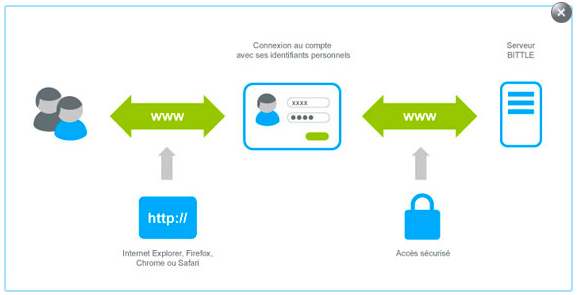
\includegraphics[scale= 0.6]{connexion.png}
  \caption{Protocole de connexion}
\end{center}  
\end{figure}
\subsubsection{Indicateurs}
L'utlisateur doit choisir les indicateurs qu'il souhaite piloter. Il a plusieurs possibilités :
\begin{itemize}
\item[•]L’utilisateur sélectionne les indicateurs parmi la bibliothèque d’indicateurs standard proposée par bittle. L’utilisateur met à disposition ses données brutes afin d’alimenter les indicateurs choisis. La solution bittle établit, de façon automatique, les liens (mapping) entre les données brutes et les indicateurs choisis.
\item[•]L’utilisateur envoie un fichier de données brutes à bittle. Celui-ci est analysé, et les indicateurs de la bibliothèque pouvant être alimentés par ces données sont mis en évidence et proposés à l’utilisateur.
\item[•]Bittle offre également la possibilité de créer ses propres indicateurs. Ainsi, l’utilisateur choisit lui-même les données nécessaires et les règles de calcul correspondantes. 
\end{itemize} 

\begin{figure}[H]
\begin{center}
  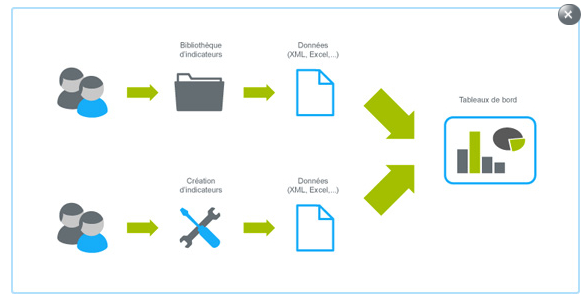
\includegraphics[scale= 0.6]{indicateur.png}
  \caption{Protocole pour le choix d'indicateurs}
\end{center}  
\end{figure}

\subsubsection{Chargement des données}
Le chargement des données pour alimenter les indicateurs de performance sélectionnés peut se faire de plusieurs manières :
\begin{itemize}

\item[•]\textbf{DataAnalyser : } traitement automatique ou manuel des fichiers csv, excel ou xml issus de n’importe quelle application source.

\begin{figure}[H]
\begin{center}
  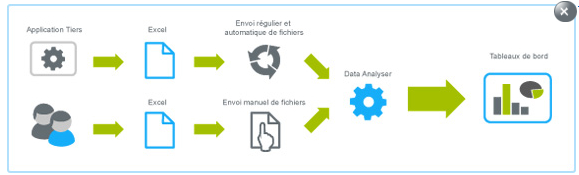
\includegraphics[scale= 0.6]{dataAnalyser.png}
  \caption{Protocole DataAnalyser pour le chargement des données}
\end{center}  
\end{figure}

\item[•]\textbf{DataMailAnalyser : } possibilité d’envoyer des données par email si l’application source dispose de cette fonctionnalité. Le contenu de ce dernier sera ensuite analysé par notre module.

\begin{figure}[H]
\begin{center}
  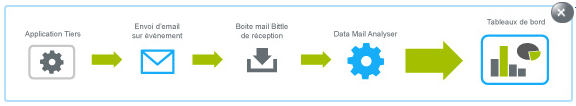
\includegraphics[scale= 0.6]{dataMailAnalyser.png}
  \caption{Protocole DataMailAnalyser pour le chargement des données}
\end{center}  
\end{figure}

\item[•]\textbf{WebAnalyser :}  communication avec des applications tierces via des Web Services.

\begin{figure}[H]
\begin{center}
  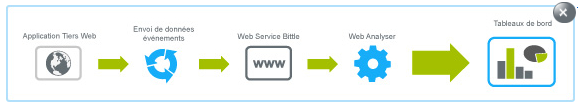
\includegraphics[scale= 0.6]{webAnalyser.png}
  \caption{Protocole WebAnalyser pour le chargement des données}
\end{center}  
\end{figure}

\end{itemize}

\subsubsection{Tableaux de bord, rapport et partage}
Bittle permet de visualiser ses données dans des tableaux de bord, via des indicateurs de performance personnalisables. Ces indicateurs peuvent ensuite être analysés globalement ou en détail, sur une période définie par l’utilisateur. Les tableaux de bord ainsi obtenus peuvent ensuite être partagés, envoyés par email ou exportés pour être intégrés dans une présentation annexe.

\begin{figure}[H]
\begin{center}
  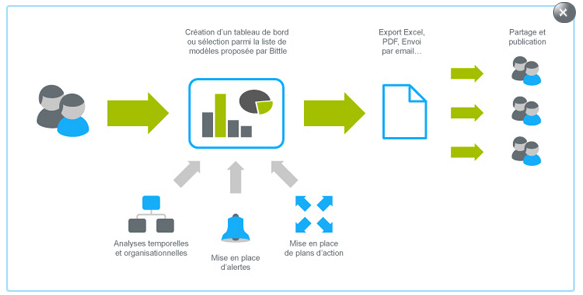
\includegraphics[scale= 0.6]{tableau.png}
  \caption{Protocole pour l'obtention de tableaux de bord}
\end{center}  
\end{figure}

\subsection{Avantages, Inconvénients de la solution}
\subsubsection{Avantages de la solution}
La solution Bittle présentée ci dessus présente de nombreux points forts par rapport aux autres offre du marché :
 
\begin{itemize}
\item[•]Absence de logiciel : cette solution ne nécessite aucune installation de logiciel sur les postes.
\item[•]Accessibilité : comme il s'agit d'une solution web, il est possible d'y accéder partout des lors qu'il y a une connexion internet.
\item[•]Coût : c'est une solution abordable pour les PME car comme annoncé plus haut cette solution coûte environ 150 €/mois/utilisateur.
\item[•]Maintenance : La maintenance du site est transparente pour les utilisateur.
\item[•]Sécurité : Bittle utilise les technologie mise en place par google.
\item[•]Collaboratif : il est possible de partager les données entre plusieurs utilisateurs.
\end{itemize}

\subsubsection{Inconvénients de la solution}

\begin{itemize}
\item[•]Limité : cette solution est limitée car elle permet uniquement de faire du reporting et des tableaux de bords. Bien qu'elle s'étende aux différents coeur de métier d'une entreprise, elle ne permet pas de faire par exemple du data mining.
\item[•] Fiabilité : c'est une solution est peu utiliser actuellement on peut se demander si elle est fiable, de plus elle utilise la technique du cloud computing, elle stock donc les données sur des serveurs externes.
\item[•]Internet : Bittle nécessite une connexion internet
\item[•]Compatibilité: elle n'est pas utilisable sur tout les navigateurs uniquement sur firefox, chrome et internet explorer.
\end{itemize}
%\newpage

\end{document}
